\subsection{UC19 - Abilitazione del plugin}
\begin{figure}[H]
	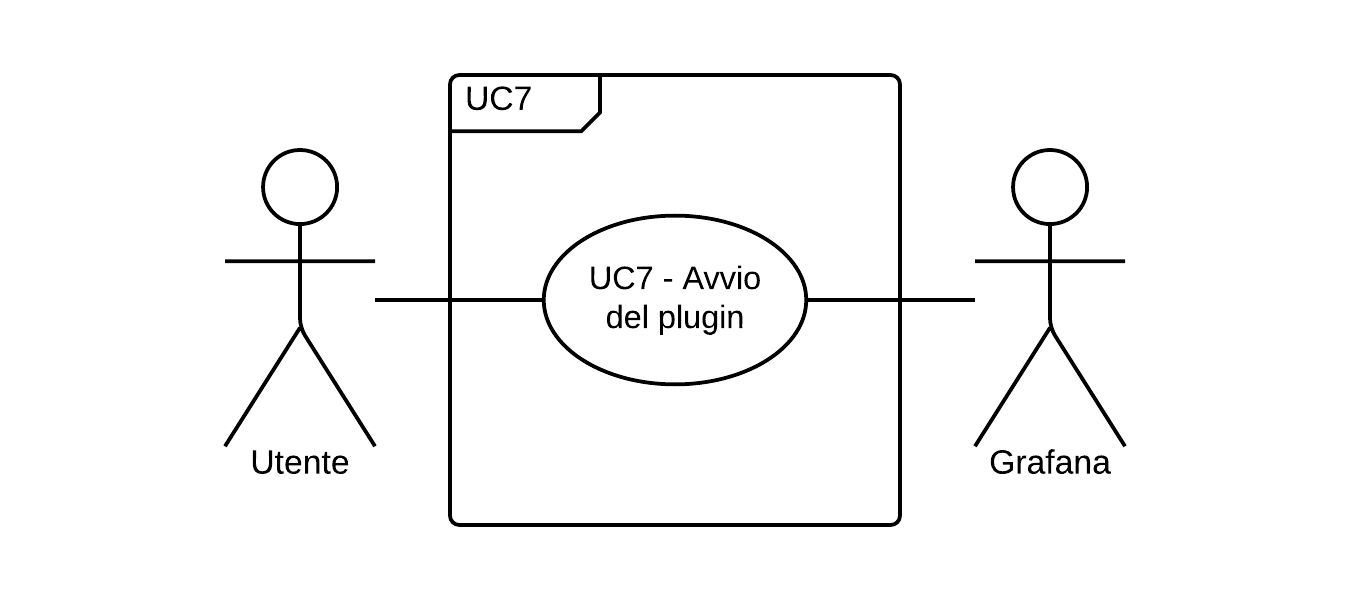
\includegraphics{img/UC7_-_Avvio_plugin.png}
	\caption{Diagramma degli use case di UC7}
\end{figure}
\begin{itemize}
	\item \textbf{Codice identificativo}: UC19;
	\item \textbf{Titolo}: abilitazione del plugin;
	\item \textbf{Attori primari}: utente;
	\item \textbf{Attori secondari}: Grafana\glo;
	\item \textbf{Descrizione}: l'utente esegue l'attività di abilitazione del plugin dalle impostazioni di Grafana\glo;
	\item \textbf{Precondizioni}: l'utente è autenticato nel sistema software Grafana\glo;
	\item \textbf{Postcondizioni}: il plug-in è stato abilitato correttamente;
	\item \textbf{Scenario principale}: l'utente accede alle impostazioni di Grafana\glosp ed abilita il plug-in. In questo modo esso viene abilitato e sarà possibile utilizzarlo aggiungendo il suo pannello alle dashboard\glosp di Grafana\glo.
\end{itemize}

\subsection{UC7 - Avvio del plug-in}
\begin{figure}[H]
	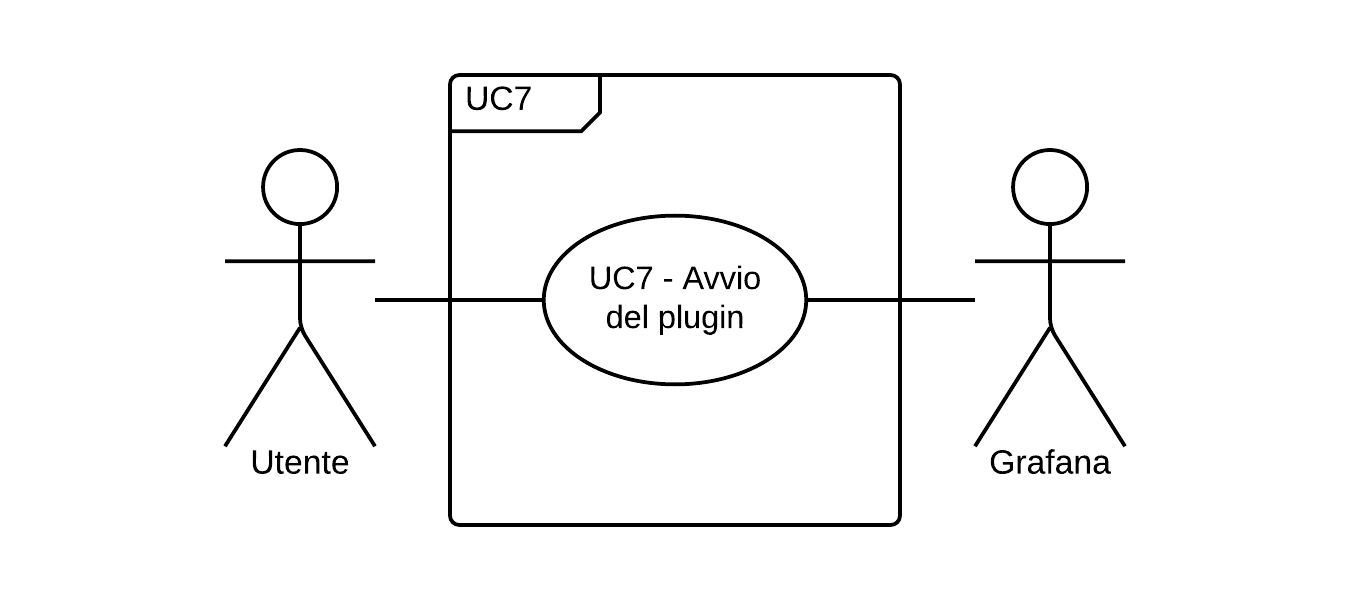
\includegraphics{img/UC7_-_Avvio_plugin.png}
	\caption{Diagramma degli use case di UC7}
\end{figure}
\begin{itemize}
	\item \textbf{Codice identificativo}: UC7;
	\item \textbf{Titolo}: avvio del plug-in;
	\item \textbf{Attori primari}: utente;
	\item \textbf{Attori secondari}: Grafana\glo;
	\item \textbf{Descrizione}: l'utente esegue l'attività di avvio del plug-in che consiste nel collegamento del pannello da esso fornito ad una dashboard\glosp configurata dall'utente;
	\item \textbf{Precondizioni}: l'utente è autenticato nel sistema software Grafana\glo, ha abilitato il plguin ed ha creato e configurato una dashboard\glosp per la visualizzazione del risultato;
	\item \textbf{Postcondizioni}: il plug-in è stato avviato correttamente;
	\item \textbf{Scenario principale}: l'utente accede alla dashboard\glosp e collega il pannello fornito dal plug-in. In questo modo esso viene avviato.
\end{itemize}
